\documentclass[11pt,a4paper]{article}

\usepackage[margin=2.2cm]{geometry}
\usepackage{amsmath,amssymb}
\usepackage{graphicx}
\usepackage{booktabs}
\usepackage{caption}
\usepackage{subcaption}
\usepackage{xcolor}
\usepackage{listings}
\usepackage[hidelinks]{hyperref}
\usepackage{enumitem}
\usepackage{parskip}
\setlist{topsep=2pt,itemsep=1pt,parsep=0pt}

\definecolor{codebg}{rgb}{0.97,0.97,0.97}
\definecolor{codekey}{rgb}{0.10,0.20,0.55}
\definecolor{codecmt}{rgb}{0.30,0.50,0.30}
\definecolor{codestr}{rgb}{0.55,0.20,0.20}
\lstset{
  basicstyle=\ttfamily\footnotesize,
  backgroundcolor=\color{codebg},
  keywordstyle=\color{codekey}\bfseries,
  commentstyle=\color{codecmt}\itshape,
  stringstyle=\color{codestr},
  showstringspaces=false,
  breaklines=true,
  frame=single,
  framerule=0pt,
  numbers=left,
  numberstyle=\tiny\color{gray},
  xleftmargin=2em,
  language=Python
}

\title{\vspace{-2.5em}\textbf{Food Recipe Provenance Classification}}
\author{}
\date{}

\begin{document}
\maketitle
\vspace{-3em}

\section{Problem and data}

The task is binary classification: predict whether each of $1734$ test recipes is American
($y{=}1$) or Italian ($y{=}2$), given $40$ TF-IDF--scored ingredient columns
($\texttt{salt}, \texttt{sugar}, \ldots, \texttt{pepper}$). The training set contains $3200$
labelled recipes. Scoring is the total misclassification count (lower is better).

\subsection{Pre-computed TF-IDF.} 

Each cell $x_{ij}=\mathrm{TF}_{ij}\cdot\mathrm{IDF}_j$ is
provided pre-computed. 

The problem statement specifies
$\mathrm{IDF}_j=\log\!\left(\frac{N}{n_j}\right)$. A direct check, however, shows this is not the
formula used: under plain-log IDF, the implied TF values $\frac{x_{ij}}{\mathrm{IDF}_j}$
within a recipe do not sum to $1$, as fractional normalization requires. Replacing the IDF with the smoothed variant $\log!\left(1+\frac{N}{n_j}\right)$ fixes this (row sums equal exactly $1$), with the recovered TF term turning out to be $\frac{1}{m_i}$ uniformly across all present ingredients, where $m_i$ is the ingredient count of recipe $i$. This is
confirmed to machine precision ($\max|\text{residual}|<10^{-13}$) across all non-zero entries of the $4934\times 40$ matrix. 

The verified formula is
$ x_{ij} = \frac{1}{m_i} \cdot \log\!\left(1+\frac{N}{n_j}\right)$, where N=4934 and $n_j$ is the count of recipes containing ingredient $j$. 

The log1p form also prevents
a degenerate case: under plain-log, any ingredient present in \emph{every} recipe receives
$\mathrm{IDF}=0$ and becomes entirely invisible. In effect, each non-zero entry encodes two things: ingredient presence and that ingredient's corpus-wide rarity via the IDF weight (common ingredients receive lower weights, rare ones higher).

\subsection{What the EDA reveals before modelling}

\textbf{(i) Sparsity and balance.} About $81.6\%$ of feature cells are zero; the median
recipe lists $7$ ingredients. The label distribution is nearly balanced: $51.5\%$ American,
$48.5\%$ Italian. Because the classes are similar in size, plain accuracy and class-weighted
loss behave very similarly, so the model is validated on misclassification count.

\textbf{(ii) Duplicate structure and an irreducible-error floor.} The $3200$ training rows
collapse into $1923$ distinct $40$-tuples; $54\%$ of test rows ($930/1734$) match a training
row exactly. Among the training duplicates, $23$ tuples carry both labels, accounting for
$195$ rows. The optimal (Bayes) prediction on each conflicting tuple is its majority label,
which still misclassifies the minority members. A direct count gives $43$ such minority rows ($1.34\%$ of the $3200$): since they share
their $40$-tuple with an oppositely labelled row, no classifier acting only on these
features can separate them. This establishes positive conditional entropy $H(Y\mid X_{40})>0$ for some patterns: the $40$ features do not uniquely
determine the label. Of the $1734$ test rows, $94$ fall on these $23$ conflicted tuples;
the lookup assigns the majority training label to all $94$, so any carrying the minority
label are irreducibly misclassified, though the exact count is unobservable without test labels.

\textbf{(iii) Univariate class signal is weak.} Figure
\ref{fig:ingdiff} shows the class-mean TF-IDF differences. The strongest single
ingredient, \texttt{flour}, has the largest Italian-side gap; \texttt{white.meat} and
\texttt{water} are comparably strong on the American side. Most features separate the classes by far less. Even ingredients commonly associated with
Italian cooking carry little signal, for instance \texttt{garlic} is marginally
\emph{more} frequent in American recipes here. The signal the classifier uses on genuinely novel recipes is therefore \emph{joint
co-occurrence} of ingredients, not any individual one.

\begin{figure}[h]
\centering
\begin{subfigure}{0.5\textwidth}
  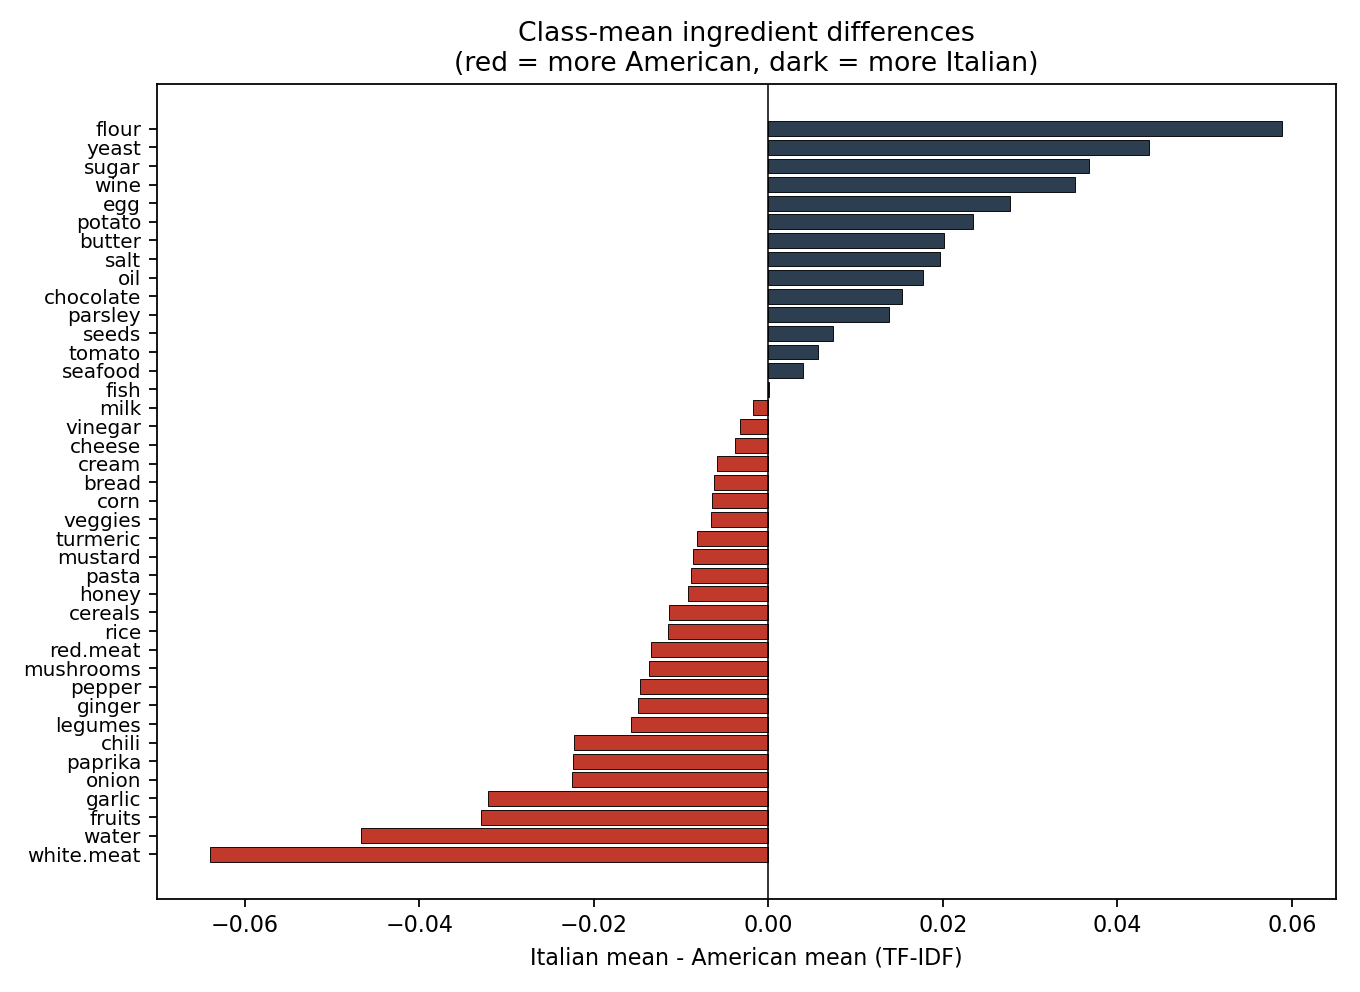
\includegraphics[width=\linewidth]{fig/fig_ingredient_diff.png}
  \caption{Italian-mean minus American-mean TF-IDF for the $40$ ingredients, sorted.}
  \label{fig:ingdiff}
\end{subfigure}\hfill
\begin{subfigure}{0.40\textwidth}
  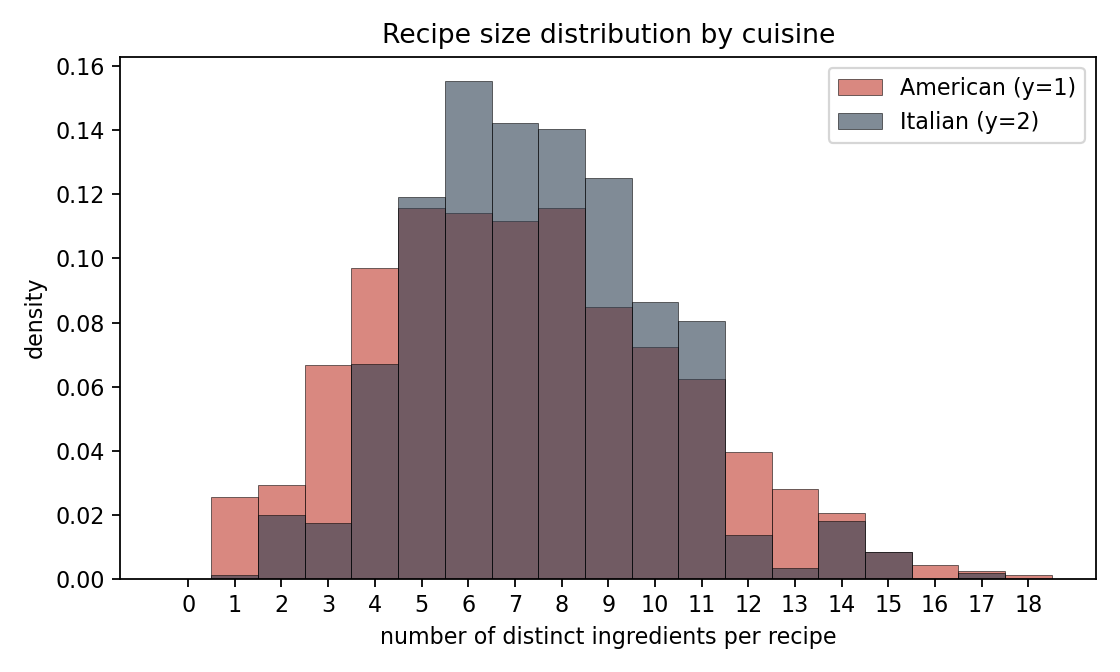
\includegraphics[width=\linewidth]{fig/fig_n_ingredients.png}
  \caption{Recipe-size distribution by class. Italian recipes have a slightly larger
  mass around $6$--$9$ ingredients; very short and very long recipes lean American.}
  \label{fig:nsize}
\end{subfigure}
\caption{Two views of the training data.}
\end{figure}

\textbf{(iv) Row-aggregate quantities carry weak but real class signal.} Beyond the $40$
columns themselves, a few simple per-recipe aggregates differ measurably between the
cuisines (Table~\ref{tab:aggr}). 

None of these classifies well on its own as the class
means overlap heavily. However, the consistent pattern is in \emph{dispersion} rather than
location: on every aggregate the American class is the more variable one. This spread
difference motivates adding the aggregates as explicit features; whether they actually earn
their place is settled by cross-validation in Section~\ref{sec:method}, not by these
marginal gaps alone.

\begin{table}[h]
\centering\small
\begin{tabular}{llcccc}
\toprule
aggregate & description & Am.\ mean & It.\ mean & Am.\ sd & It.\ sd \\
\midrule
\texttt{total\_mass}     & row sum $\sum_j x_{ij}$                 & $1.63$ & $1.55$ & $0.27$ & $0.17$ \\
\texttt{mean\_intensity} & total mass per ingredient               & $0.31$ & $0.24$ & $0.31$ & $0.11$ \\
\texttt{n\_ingredients}  & distinct ingredients $|\{j:x_{ij}>0\}|$ & $7.20$ & $7.50$ & $3.24$ & $2.57$ \\
\bottomrule
\end{tabular}
\caption{Per-recipe aggregate features by cuisine.}
\label{tab:aggr}
\end{table}


\section{Path to the final solution}

All major classifier families were evaluated on the same grouped cross-validation
protocol described below; Table~\ref{tab:models} maps the landscape from the simplest to
most expressive models.

\paragraph{A note on validation.}
Because $54\%$ of test patterns also appear in training (Section~1, point~(ii)), standard
$k$-fold cross-validation would place copies of the same recipe in both training and test
folds: the model could recall those test rows by memory rather than by generalising. Hence $1679$ duplicate rows are
always placed in training; only $1521$ singleton rows (whose feature vector is unique) rotate across folds as the test set. Because no singleton's $40$-tuple ever appears in the training portion of its fold, every test
prediction must generalise to a genuinely new recipe. Five repetition of $3$-fold CV on the
singleton rows give $15$ independent error estimates (each on $\approx 507$ novel recipes);
Table~\ref{tab:models} reports their mean and standard deviation.

\begin{table}[h]
\centering\small
\begin{tabular}{lcc}
\toprule
Method & Error\,(\%) & Std\,(\%) \\
\midrule
Complement Naive Bayes & $29.15$ & $2.17$ \\
LDA & $27.32$ & $1.65$ \\
Bernoulli Naive Bayes & $26.63$ & $2.04$ \\
\addlinespace[4pt]
Logistic regression (L2) & $26.43$ & $1.59$ \\
Logistic regression (elastic net) & $26.40$ & $1.63$ \\
Logistic regression (L1) & $26.36$ & $1.57$ \\
\addlinespace[4pt]
KNN (cosine, $k{=}5$) & $23.20$ & $1.30$ \\
\addlinespace[4pt]
XGBoost & $16.48$ & $1.65$ \\
LightGBM & $16.34$ & $1.55$ \\
HistGradientBoosting & $16.33$ & $1.28$ \\
\addlinespace[4pt]
SVM (RBF kernel) & $14.81$ & $1.45$ \\
\addlinespace[4pt]
Random forest & $14.32$ & $1.36$ \\
Extra-Trees (43 features, final) & $12.83$ & $0.74$ \\
Extra-Trees (40 features) & $12.73$ & $1.00$ \\
\bottomrule
\end{tabular}

\caption{Novel-row error: grouped cross-validation ($5\times 3$-fold on singleton rows,
$n\approx507$ per fold) on the raw $40$ features, except the final Extra-Trees row which
also shows the $43$-feature variant. Error is mean misclassification rate; Std is the
fold-to-fold standard deviation. Within each group and across groups: ordered worst to best.}
\label{tab:models}
\end{table}

\textbf{\textit{LDA}} and the \textbf{\textit{Naive Bayes}} variants perform worst among the simpler probabilistic and linear-style methods: the Gaussian
within-class assumption underlying LDA is violated by a feature matrix that is $81.6\%$
zero, and QDA is not pursued because its per-class $40\times40$ covariance matrices are
near-singular under the same sparsity. Bernoulli and Complement Naive Bayes are similarly
limited by their independence assumption between ingredients.

\textbf{\textit{Logistic regression}} with L2, L1, and elastic-net penalties gives errors within $0.1$\,pp
of one another (Table~\ref{tab:models}), well within the $\sim\!1.6$\,pp fold-to-fold
standard deviation. Regularisation type has no material effect because the bottleneck is not
overfitting but the linear decision boundary itself, which cannot represent the joint
ingredient co-occurrences the EDA identified as the main signal.

\textbf{\textit{$k$-NN}} improves on linear methods, but pairwise distances in a $40$-dimensional sparse
space are less discriminative and cannot capture the higher-order co-occurrence structure
that separates the cuisines.

\textbf{\textit{RBF SVM}}\footnote{The RBF (Radial Basis Function) kernel maps inputs to an infinite-dimensional space via
Gaussian proximity, allowing non-linear boundaries without computing the feature map
explicitly. Implemented as \texttt{SVC} in scikit-learn; $C$ and $\gamma$ were tuned
via the grouped cross-validation described above.} reaches $14.81\%$, improving over
linear methods and $k$-NN. The kernel implicitly embeds the sparse input vectors into a
space where ingredient co-occurrence patterns become more linearly separable---the gain
over linear classifiers. It still falls below both forest methods.

\textbf{\textit{Gradient-boosted trees}}\footnote{
Gradient boosting fits $M$ trees sequentially, each 
targeting the pseudo-residuals 
$r_{im} = -\bigl[\frac{\partial L(y_i, f(x_i))}{\partial f(x_i)}\bigr]_{f=f_{m-1}}$, 
with per-leaf weights $\gamma_{jm}$ found by line search.
The implementations here extend this as follows:
\begin{itemize}
\item \emph{XGBoost} replaces the per-leaf line search with a Newton step using
both the gradient
$g_i = \bigl[\frac{\partial L(y_i, f(x_i))}{\partial f(x_i)}\bigr]_{f=f_{m-1}}$
and Hessian
$h_i = \bigl[\frac{\partial^2 L(y_i, f(x_i))}{\partial f(x_i)^2}\bigr]_{f=f_{m-1}}$.
For leaf $j$ with index set $I_j$, let
$G_j = \sum_{i \in I_j} g_i$ and $H_j = \sum_{i \in I_j} h_i$;
the optimal leaf weight is then $w_j^* = -\frac{G_j}{H_j + \lambda}$,
where $\lambda$ is an $\ell_2$ penalty on leaf weights.
This yields a Newton-style update and regularises tree complexity to
limit overfitting.

\item \emph{LightGBM} grows trees \emph{leaf-wise}: instead of expanding 
the tree level by level, it repeatedly splits the leaf that gives the 
largest reduction in loss. It also uses two computational shortcuts. 
\emph{GOSS} (Gradient-based One-Side Sampling) keeps observations with 
large $|r_{im}|$, because these are the observations the current model 
fits poorly, and samples only a subset of observations with small 
$|r_{im}|$. \emph{EFB} (Exclusive Feature Bundling) combines sparse 
features that are rarely non-zero at the same time, reducing the number 
of features over which split searches are performed.

\item \emph{HistGradientBoosting} speeds up split search by grouping each continuous feature into a 
small number of ordered bins. Instead of testing all possible thresholds 
of $x_j$, the algorithm maps values into bin labels
$\tilde{x}_j \in \{1,\ldots,255\}$.
A split $\tilde{x}_j \leq k$ corresponds to splitting at the boundary 
between two ordered intervals of the original variable, so the algorithm 
compares at most $255$ bin thresholds rather than all observed feature 
values.
\end{itemize}
}
(XGBoost, LightGBM, HistGradientBoosting) reach $16.3\%$--$16.5\%$ error---counter-intuitively worse than SVM and below both forest methods. A natural intuition is that sparse
features cause this, but XGBoost has explicit sparsity-aware split finding and is generally
strong on sparse data. The likelier reason is small sample size: with only $3200$ rows,
weak per-feature signal and high zero-inflation, sequential residual fitting tends to
memorise the few informative interactions early and then chase noise. Extra-Trees' double
layer of randomisation (random feature subset \emph{and} random split thresholds) yields
trees that are individually weaker but decorrelated, and the averaged prediction has lower
variance, which is a better fit to this regime.

Tree ensembles that grow each tree independently and then average them sidestep the
sequential-fitting bottleneck. \textbf{\textit{Random Forests}} decorrelate trees by
restricting each split to a random feature subset, improving substantially over gradient
boosting ($14.3\%$ vs $16.3\%$--$16.5\%$). \textbf{\textit{Extra-Trees}}\footnote{Extra-Trees
(``extremely randomised trees'', Geurts, Ernst \& Wehenkel, 2006) is a variant of random
forests described in detail in Section~\ref{sec:method}.} adds a second randomisation:
split thresholds are drawn at random from the feature's range rather than optimised, which
further decorrelates the trees. It is the best-performing family at $12.7\%$ on raw features.
Table~\ref{tab:models} benchmarks all families on the raw $40$ features to keep the
cross-family comparison on equal footing. The engineered aggregates from Section~1 are
evaluated separately for Extra-Trees only, shown as two rows. The $0.10$\,pp difference
in mean error ($12.73\%\to12.83\%$) is within fold-to-fold noise, but the fold-to-fold
standard deviation drops from $1.00\%$ to $0.74\%$---a $26\%$ reduction. This is the
payoff Section~1 anticipated: the aggregates do not carry new information the trees
cannot eventually reconstruct from the raw columns, but supplying them explicitly as
columns allows depth-$1$ splits to capture recipe-level magnitude directly, removing a
source of fold-to-fold variance. ET-$43$ is therefore chosen as the final model.

A stacking ensemble was then tried on the raw $40$ features, combining SVM-RBF,
Extra-Trees, and three gradient-boosting variants as \emph{base learners}. Each base learner
produces a predicted class probability; the five probabilities are concatenated into a
$5$-dimensional vector and passed as input to a \emph{meta-learner} - a logistic regression
that learns a weighted combination of those probability estimates.\footnote{Training the meta-learner on out-of-fold
predictions rather than in-sample predictions ensures its weights are estimated on held-out
data, preventing it from simply memorising the base learners' training errors.} The grouped cross-validation described above gave the
stack and a single multi-seed Extra-Trees the same novel-row error ($12.85\%$ vs
$12.79\%$; difference well within fold-to-fold noise). The stack's added complexity brought no measurable accuracy on the part of the test set
that the model actually has to predict (the $46\%$ of test rows whose pattern is not in
training).

The simpler model was chosen: a multi-seed Extra-Trees on $43$ features (the $40$ raw
columns plus the three row aggregates), combined with a \emph{lookup} step that returns the
training majority label whenever a test row's $40$-tuple appears in training. For duplicate-matched test rows a leave-one-out estimate gives $\sim 97\%$ accuracy ($43$ of $1679$ duplicate training rows are unavoidable minority misclassifications from
the $23$ conflicted tuples). For singleton-matched rows the lookup is deterministic (one
unambiguous training label), so errors can arise only from labelling noise, not from the
classification problem itself. Since $930$ test rows match a training pattern (Section~1, point~(ii)), the lookup
covers roughly half the predictions at accuracy well above the $\sim 87\%$ the classifier
achieves on genuinely novel rows.

\section{Final method}
\label{sec:method}

The final pipeline has two components: an \emph{exact-pattern lookup} and an
\emph{Extra-Trees} classifier. 

\subsection{Exact-pattern lookup}

Build a dictionary keyed by the $40$-tuple of every training row. For each key, store the
majority training label. Predict any test row whose $40$-tuple is in the dictionary with
that majority label.

In the training set $1923$ distinct $40$-tuples cover the $3200$ rows; $1900$ tuples are
unanimous and $23$ are conflicted. On test, $930$ tuples match (Section~1, point~(ii)).
This is a direct application of the Bayes' rule in the finite-feature-space limit: with no
further information than the $40$-tuple, the class-conditional probability is estimated by
the training proportion, and the optimal $0$--$1$ prediction is the empirical mode.

\subsection{Extra-Trees on engineered features}

\paragraph{About Extra-Trees.} Extra-Trees is a small variation on random forests, adopted here after empirical
comparison.

Bagging fits $B$ trees on bootstrap samples and averages them: $\hat f_{\mathrm{bag}}(x) = \tfrac{1}{B}\sum_{b=1}^{B}\hat f^{(b)}(x)$.
Averaging lowers variance, but the bootstrap trees remain correlated because they keep
finding the same strong splits. Random forests reduce that correlation by restricting each
split to a random subset of $m\!\ll\!p$ features. The variance of the average of $B$
identically distributed predictors with pairwise correlation $\rho$ is
$\mathrm{Var}(\bar f) \;=\; \rho\,\sigma^{2} + \tfrac{1-\rho}{B}\,\sigma^{2}$,
so decreasing $\rho$ pushes the variance towards $\rho\,\sigma^2$ instead of $\sigma^2$.

Extra-Trees adds a second source of randomness: for each candidate feature considered at a
split, the threshold is \emph{drawn at random} from the feature's empirical range instead
of being chosen to minimise impurity. 

Furthermore Extra-Trees does \emph{not} bootstrap;
each tree is fit on the full training data. 

The two changes have complementary effects:
random thresholds further decorrelate the trees (lower $\rho$), and using all $3200$ rows
in every tree slightly lowers the per-tree variance ($\sigma^2$).

\paragraph{Hyperparameters and tuning.} The final model uses \texttt{n\_estimators}$=600$,
\texttt{max\_features}$=\sqrt{p}$ (where $p=43$, so $7$ features considered per split),
\texttt{min\_samples\_leaf}$=1$, \texttt{max\_depth}$=\mathrm{None}$. A sweep was run over
each of these: raising \texttt{min\_samples\_leaf} (in $\{1,2,3,5,8,12,20\}$), capping
\texttt{max\_depth} (down to $10$), and raising \texttt{max\_features} (to $0.3$, $0.5$,
$0.7$, $1.0$). Every regularising change \emph{hurt} cross-validation accuracy. The
explanation is internal to Extra-Trees: regularising individual trees increases their
correlation, which is the quantity the ensemble works to reduce. The randomness in the
splits is already a strong form of regularisation; further regularising the base learner
defeats the design.

\paragraph{Multi-seed averaging.} The same Extra-Trees forest is fit under $30$ different
random seeds and the class probabilities are averaged before taking the argmax. Each seed
gives a different realisation of the random feature subsets and split thresholds. The
accuracy gain from $1$ seed to $30$ is small ($+0.09$ percentage points in honest
cross-validation), but the cost is only a constant factor on the final training run, and
the variance of the ensemble output across seeds drops from $\sim 0.0007$ to negligible.

\paragraph{Engineered features.} In addition to the $40$ raw TF-IDF columns the model
appends
\[
n_{\mathrm{ingredients}} = \sum_j \mathbf{1}\{x_{ij}>0\}, \quad
\mathrm{total\_mass} = \sum_j x_{ij}, \quad
\mathrm{mean\_intensity} = \frac{\mathrm{total\_mass}}{n_{\mathrm{ingredients}}}.
\]
These are deterministic functions of the $40$ columns; they do not add information, but
their explicit presence lets the trees split on row-level aggregates with depth $1$
instead of depth $\approx 6$, which lowered cross-validation variance. The class signal
of each was checked in the EDA (Table~\ref{tab:aggr}); \texttt{std\_intensity} was left
out, its separation being the weakest of the candidates and an honest-cross-validation
test unable to distinguish it from no feature at all.

\subsection{Combining the two predictors}

For each test row:
\begin{enumerate}
  \item If the $40$-tuple appears in the training dictionary, output the training majority
        label.
  \item Otherwise, output the argmax of the $30$-seed-averaged Extra-Trees probability.
\end{enumerate}
This routes $930/1734=53.6\%$ of test predictions through the lookup and the remaining
$804$ through the model.

\section{Feature importance and what the model uses}

The trained Extra-Trees is interpreted with two complementary tools: (i)
\emph{Gini importance} (mean decrease in impurity across all splits using a feature),
standard for tree ensembles and (ii) \emph{SHAP}
(SHapley Additive exPlanations\footnote{Lundberg \& Lee, ``A Unified Approach to
Interpreting Model Predictions'', NeurIPS 2017.

SHAP is based on Shapley values from cooperative game theory, where features are treated
as ``players'' and the model prediction is the ``payoff'' to be fairly divided among them.
For a given observation $x$, SHAP starts from the model's average prediction
$E[\hat f(X)]$ and explains how each feature moves the prediction toward $\hat f(x)$.
Each feature $j$ receives a value $\phi_j$: if $\phi_j>0$ it pushes the prediction above
average; if $\phi_j<0$ it pulls it below. The magnitude of $\phi_j$ shows how strongly
that feature contributes, and the values are additive:
$\sum_{j=1}^p \phi_j = \hat f(x) - E[\hat f(X)]$, so the full gap between the individual
and average prediction is exactly accounted for. 

Computing exact Shapley values requires
evaluating all $2^p$ feature subsets; \emph{TreeSHAP} exploits the tree structure for
exact values in $O(TLD^2)$ time ($T$ trees, $L$ maximum leaves, $D$ maximum depth), and
is applied here to the entire training set with one seed.}).

\begin{figure}[h]
\centering
\IfFileExists{fig/fig_shap_summary.png}{
  \begin{subfigure}{0.48\textwidth}
    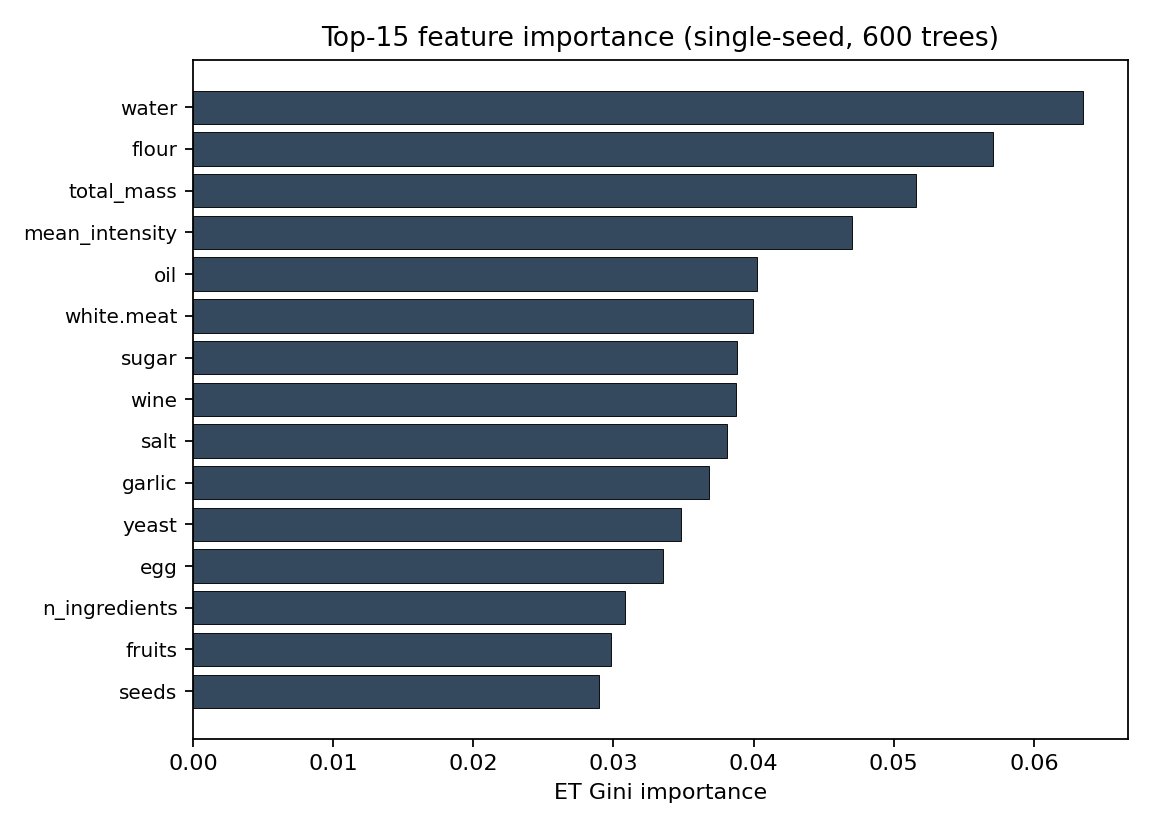
\includegraphics[width=\linewidth]{fig/fig_feature_importance.png}
    \caption{Gini importance, top $15$ features.}
    \label{fig:gini}
  \end{subfigure}\hfill
  \begin{subfigure}{0.50\textwidth}
    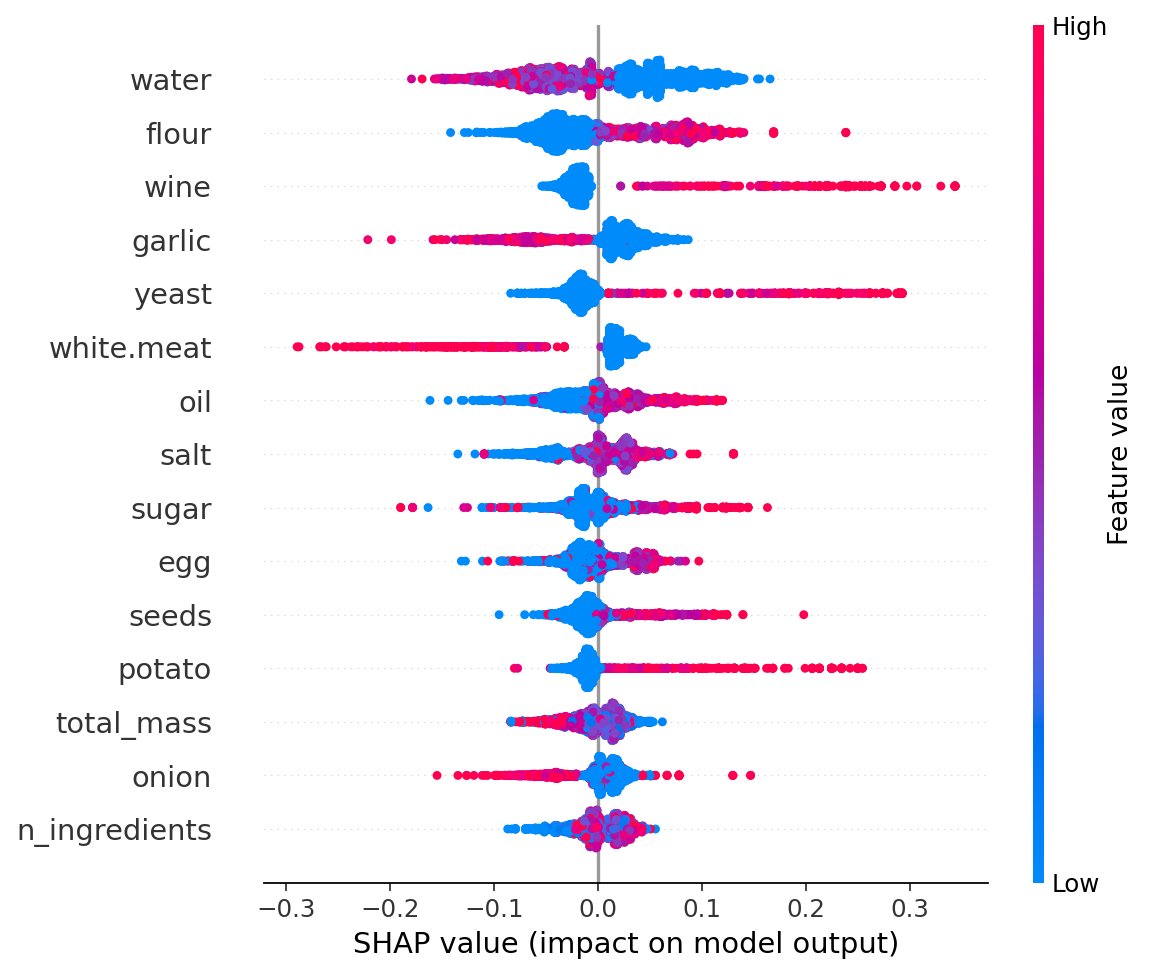
\includegraphics[width=\linewidth]{fig/fig_shap_summary.png}
    \caption{TreeSHAP summary, top $15$ features. Each point is
    one recipe; horizontal position is the SHAP value (positive $=$ pushes toward Italian).}
    \label{fig:shap}
  \end{subfigure}}
{
  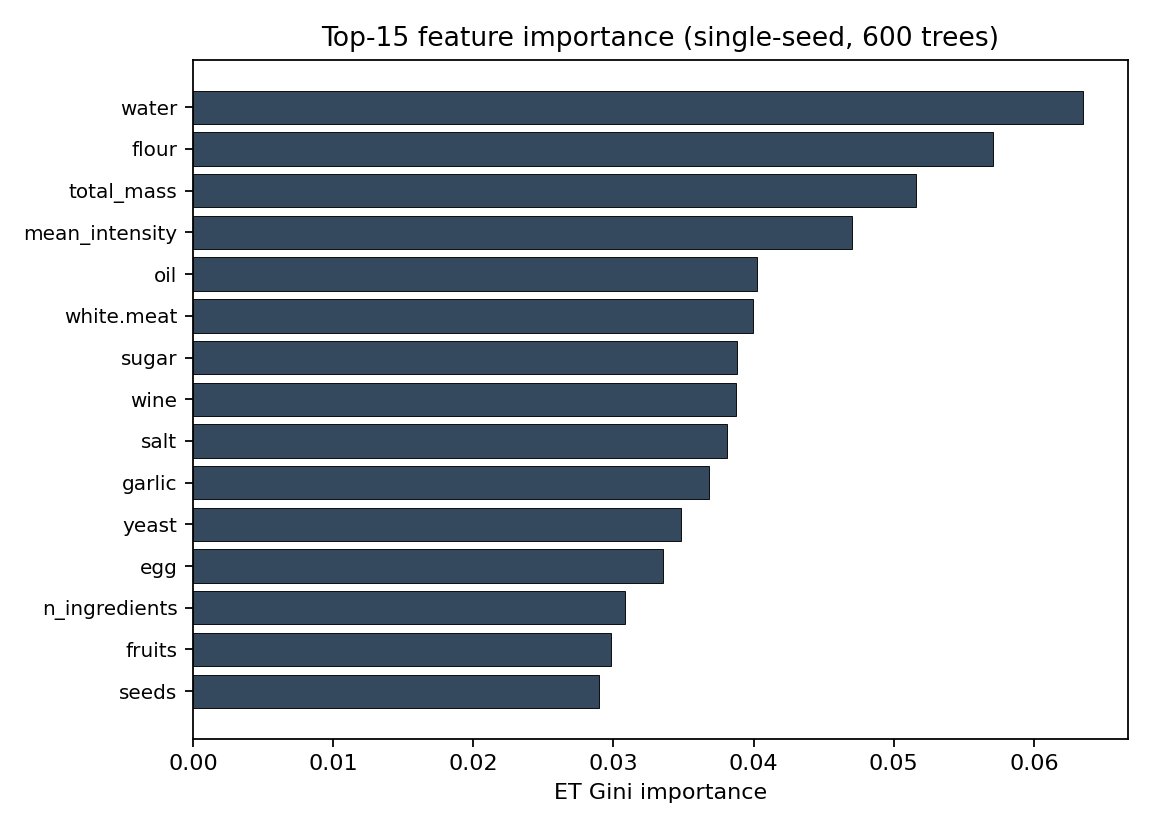
\includegraphics[width=0.62\linewidth]{fig/fig_feature_importance.png}
}
\caption{Feature importance for the final classifier. Gini importance and, where
available, the TreeSHAP summary of an Extra-Trees fit with $600$ trees and one
random seed.}
\label{fig:feature-importance}
\end{figure}

The two ranks agree on the most important features. The
top of the Gini ranking is \texttt{water}, \texttt{flour}, then the engineered
\texttt{total\_mass} and \texttt{mean\_intensity}: trees need explicit aggregate columns
to use recipe-level magnitude with depth-$1$ splits, and indeed two of the three
engineered features land in the top four. The most informative individual ingredients
that follow are \texttt{oil}, \texttt{white.meat}, \texttt{sugar}, \texttt{wine},
\texttt{salt}, \texttt{garlic}, \texttt{yeast} and \texttt{egg}, broadly consistent with
the class-mean differences in Fig.~\ref{fig:ingdiff}. The SHAP plot adds the
\emph{direction}: \texttt{flour}-, \texttt{yeast}- and \texttt{wine}-rich rows push toward
Italian, while \texttt{water}-, \texttt{white.meat}- and \texttt{garlic}-rich rows push
toward American (the last is one of the counter-stereotype findings noted in the EDA).

\textbf{Caveat.} The bijection between ingredient set and TF-IDF vector means that an
individual feature's importance understates its real informativeness, because each row's
$40$-tuple is highly correlated with the count of non-zero entries that the feature
$n_{\mathrm{ingredients}}$ captures. The plot should be read as ``what the trees route a prediction
through'' rather than as a faithful map of class relevance.

\section{Discussion and limitations}

\paragraph{Refinements that did not help.} Several further directions were tested and
rejected by grouped cross-validation.

 \textit{Feature engineering transforms}: within-group relative intensity features over
ingredient clusters (ratios, dominance indicators, and within-group entropy), and the
top-$k$ ingredient pairs ranked by class-discriminative co-occurrence (motivated by a
per-class co-occurrence heatmap that showed visually distinct patterns between the two
cuisines), all failed to improve over the baseline. The underlying reason is structural: the TF-IDF encoding is
a bijection from ingredient set to feature vector, so any derived column is in principle
already available to the Extra-Trees model at sufficient tree depth; explicit interaction
terms reduce depth requirements without adding new information. 

\textit{Pre-trained
semantic embeddings} of the ingredient names - mapping each name to a dense vector
encoding typical cuisine associations - seem promising but are confounded by the corpus
labelling: a substantial fraction of recipes labelled American are Italian-American dishes
with Italian-like ingredient lists, so an external semantic association that links Italian
ingredient names to the Italian class would push exactly those rows in the wrong direction.
Cross-validation confirmed no benefit. 

A decision-threshold sweep showed that shifting the
Extra-Trees boundary toward predicting more American increased total misclassification
monotonically, so the default $0.5$ threshold is kept.

\paragraph{What limits the accuracy.} A concrete source of irreducible error is the $23$
conflicted training tuples: the lookup predicts the majority training label, and $94$ test
rows fall on these tuples. Any of those $94$ that carry the minority label will be wrong
regardless of model quality; the exact count is not observable without the test labels. A more conceptual
limit is that the $40$ columns are themselves a coarse categorisation of real
ingredients: \texttt{cheese}, \texttt{veggies} and \texttt{red.meat} are bundles that hide
\texttt{parmesan} vs \texttt{cheddar}, \texttt{basil} vs \texttt{kale},
\texttt{bolognese} vs \texttt{steak}. Inspecting the misclassified rows shows many are
recipes a human cook would call Italian-American: pizza-dough-like or pesto-like
ingredient lists that the corpus labels American. Even an external oracle that knew the
true cuisine - ingredient mapping might disagree with these labels, so the residual error
on novel recipes is best understood as a property of the coarsened representation rather
than a modelling failure that more tuning would remove.

\section{Reproducing the submission}

The script is reproduced in full below. It depends only on \texttt{numpy},
\texttt{pandas}, and \texttt{scikit-learn}.  The two inputs are
the unmodified \texttt{train.csv} and \texttt{test.csv}; both must sit in the working
directory.

\lstinputlisting{../n02_final_model.py}

\end{document}
